\section{Milestone M0: honest noisy simulation}
\label{sec:m0}

\begin{tcolorbox}[colback=gray!5, colframe=gray!40, title={M0 at a glance}, fonttitle=\bfseries]
  \textbf{Question.} Are the noisy numbers real?\quad
  \textbf{Answer.} They were not: the simulator never sampled. After M0 the noisy floor is
  \VPostFinalMin{} to \VPostFinalMax{} (was about $-14$).\\
  \textbf{Code.} Commit \texttt{0433fd7}. \textbf{Results.} \py{results/statevector_m0-summary},
  \py{results/fake_guadalupe_m0-summary}. \textbf{Status.} Done; hardware check H0 deferred.
\end{tcolorbox}

\subsection{Goal and exit criteria}

The first noisy benchmark reported energies around $-14$ on \py{FakeGuadalupeV2}. While
diagnosing that plateau (\cref{sec:noise}), three defects in the simulation turned up. M0 had to
remove them before any method comparison could be trusted. Its exit criterion was a new noisy
baseline in the README, backed by four checks: the standard error falls as $1/\sqrt{\text{shots}}$,
identical parameter rows differ between calls, readout error alone moves the energy, and
RVB\,+\,ADAM no longer climbs.

\subsection{The three defects}

\begin{enumerate}
  \item \textbf{No sampling.} The \py{aer_ideal} and \py{aer_noisy} backends used Aer's own
    \py{EstimatorV2}, which computes expectation values with \py{save_expectation_value}
    instead of sampling. Shots had no effect, reported standard errors were zero, and readout
    error was never applied. A unit test meant to check shot noise passed vacuously.
  \item \textbf{Seed reuse made a fake gradient.} Each row of a parameter batch got a fixed
    simulator seed. Identical parameters then gave different energies per row, with the
    \emph{same} pattern on every call: a spread of \VSeedBugSpread{} across \VSeedBugRows{}
    identical rows. With finite-difference step $\varepsilon=\VFdEps$ this is a constant fake
    gradient of about \VSeedBugGrad{} per component, and ADAM followed it.
  \item \textbf{``Best energy'' was biased low.} Reporting the minimum over a noisy trace
    selects favourable fluctuations.
\end{enumerate}

The second item explains the most visible symptom, RVB\,+\,ADAM climbing from
\VPreBestRvbAdam{} to \VPreFinalRvbAdam{} (Figure~\ref{fig:m0}, right panel). SPSA was unaffected
because its random perturbation directions average a fixed per-row bias away.\footnote{The
numbers in item~2 are quoted from \py{docs/roadmap.md}, section~1.3; the code that produced
them was replaced in M0 and cannot be rerun.}

\subsection{Implementation}

\begin{itemize}
  \item \textbf{Sampling estimator.} \py{AerEnergy} now wraps
    \py{qiskit.primitives.BackendEstimatorV2} around an \py{AerSimulator} (density matrix with
    noise, statevector without). Each energy measures the \VMeasGroups{} commuting bases with the
    requested shots, so shot noise and readout error appear as on hardware.
  \item \textbf{Fresh seeds.} Every call draws a new simulator seed from the run's generator
    (\py{_next_seed}). Runs stay reproducible from the run seed, but repeated parameters no
    longer share a noise pattern.
  \item \textbf{Final re-measurement.} \py{run_vqe} re-measures the final parameters once with
    \py{backend.final_shots} (16384 per basis) and reports that as \emph{the} result; the trace
    minimum is kept only as a diagnostic.
\end{itemize}

\subsection{Results}

\begin{table}[H]
  \centering
  % Generated by `uv run python -m docsgen`; do not edit.
\begin{tabular}{lccccc}
\toprule
 & \multicolumn{2}{c}{before M0 (no sampling)} & \multicolumn{3}{c}{after M0 (sampled, re-measured)} \\
\cmidrule(lr){2-3}\cmidrule(lr){4-6}
combination & final & best of trace & final & best of trace & rel.\ error \\
\midrule
RVB + SPSA & \VPreFinalRvbSpsa & \VPreBestRvbSpsa & \VPostFinalRvbSpsa & \VPostBestRvbSpsa & \VPostErrRvbSpsa \\
RVB + ADAM & \VPreFinalRvbAdam & \VPreBestRvbAdam & \VPostFinalRvbAdam & \VPostBestRvbAdam & \VPostErrRvbAdam \\
HVA + SPSA & \VPreFinalHvaSpsa & \VPreBestHvaSpsa & \VPostFinalHvaSpsa & \VPostBestHvaSpsa & \VPostErrHvaSpsa \\
HVA + ADAM & \VPreFinalHvaAdam & \VPreBestHvaAdam & \VPostFinalHvaAdam & \VPostBestHvaAdam & \VPostErrHvaAdam \\
\bottomrule
\end{tabular}

  \caption{The noisy FakeGuadalupeV2 benchmark (the paper's four combinations) before and after
    M0. ``Final'' after M0 is the re-measured energy. All four now sit on the noise floor of
    \cref{sec:noise}; before M0 the floor looked higher because readout error was missing.}
  \label{tab:m0}
\end{table}

\begin{figure}[H]
  \centering
  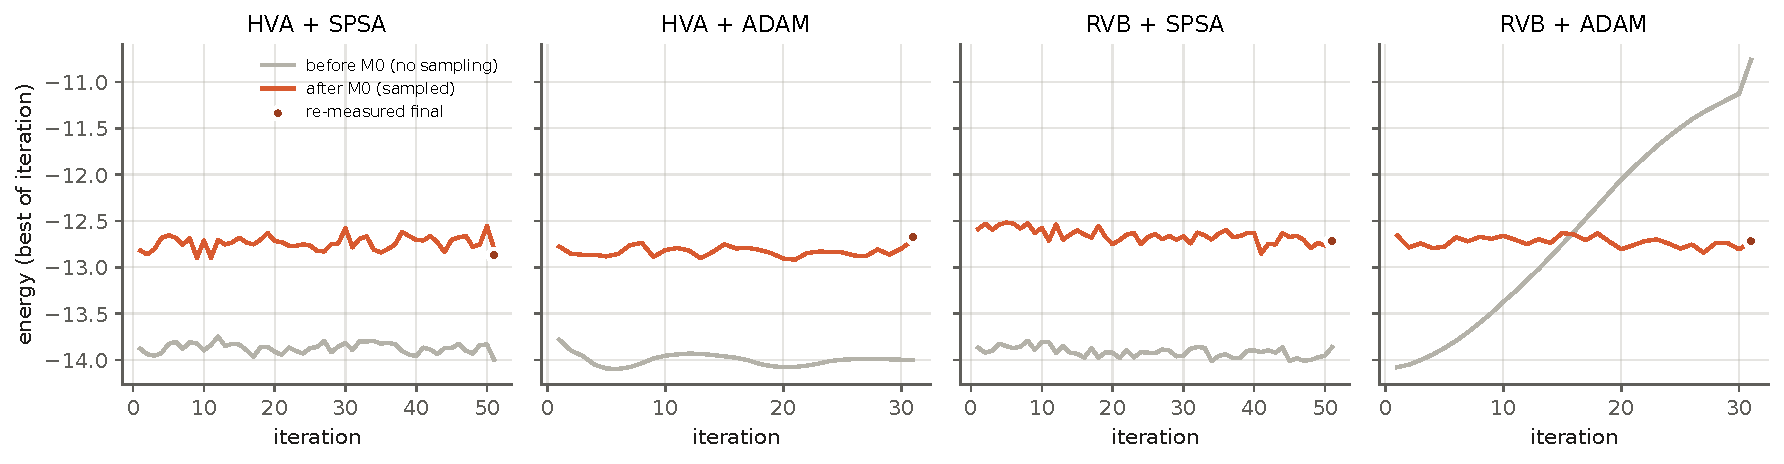
\includegraphics[width=\linewidth]{m0_before_after}
  \caption{Convergence before (grey) and after (orange) M0, best energy of each iteration. The
    upward shift of about one unit (from about $-14$ to $-12.8$) is the readout error that was
    missing: it adds bias. The climb of
    RVB\,+\,ADAM (right) is gone. Dots: the re-measured final energy.}
  \label{fig:m0}
\end{figure}

Figure~\ref{fig:m0} and Table~\ref{tab:m0} show the two effects of M0 separately. The
\emph{level} moved from about $-14$ to about $-12.8$: that is readout error, consistent with the
factor \VKeepHvaReadout{} of Table~\ref{tab:floor}. The \emph{shape} of RVB\,+\,ADAM changed from
a steady climb to a flat line: that is the fake gradient disappearing. On the exact
statevector backend nothing changed (Table~\ref{tab:m0sv}), as expected, since none of the three
defects touches exact simulation.

\begin{table}[H]
  \centering
  % Generated by `uv run python -m docsgen`; do not edit.
\begin{tabular}{lcc}
\toprule
combination & final energy & rel.\ error \\
\midrule
RVB + SPSA & \VSvFinalRvbSpsa & \VSvErrRvbSpsa \\
RVB + ADAM & \VSvFinalRvbAdam & \VSvErrRvbAdam \\
HVA + SPSA & \VSvFinalHvaSpsa & \VSvErrHvaSpsa \\
HVA + ADAM & \VSvFinalHvaAdam & \VSvErrHvaAdam \\
\bottomrule
\end{tabular}

  \caption{Exact statevector benchmark, for reference. HVA returns to zero parameters exactly;
    RVB with SPSA stops at \VSvErrRvbSpsa.}
  \label{tab:m0sv}
\end{table}

\subsection{Checks}

\begin{itemize}
  \item \emph{Standard error falls as $1/\sqrt{\text{shots}}$.} Over \VSpreadRepeats{} repeats at
    the start point, the real spread is \VSpreadLowReal{} at 1024 shots and \VSpreadHighReal{} at
    4096: a factor of two for four times the shots.
  \item \emph{Identical rows differ between calls; readout alone moves the energy}
    ($-18\to\VFloorHvaReadout$). Both are unit-tested in the package.
  \item \emph{RVB\,+\,ADAM no longer climbs}: final \VPostFinalRvbAdam.
\end{itemize}

\subsection{Findings carried forward}

\begin{rem}[The reported standard error is a bound]\label{rem:stdbound}
  The sampling primitive reports $\sum_i|c_i|\,\sigma_i/\sqrt{s}$ over the Pauli terms, which
  ignores correlations between terms. At the start point it reports \VSpreadLowReported{} at
  1024 shots against a real spread of \VSpreadLowReal{}, about \VSpreadRatio{} times too large;
  at the optimum the real spread without noise is exactly zero (\cref{prop:zerovar}). Method comparisons in M1
  and later therefore use repeated runs, never the reported \py{std}.
\end{rem}

\begin{rem}[Simulation cost]
  Noisy density-matrix simulation costs about \VSecPerEnergy{}\,s per energy regardless of the
  shot count (the density matrix is evolved once, sampling is cheap). Simulator studies can use
  large shot budgets for free; hardware cannot. This is what limited the noisy part of M1 to one
  seed and to RVB.
\end{rem}

\subsection{Problems solved and open}

\begin{itemize}
  \item[\checkmark] The three defects are fixed and covered by unit tests; the vacuous Aer test
    now asserts real shot noise.
  \item[\checkmark] New noisy baseline in the README (Table~\ref{tab:m0}).
  \item[$\circ$] \textbf{Hardware checkpoint H0 deferred} at the group's request. The IBM
    Runtime code path is kept and tested in local mode only, so the fake-backend floor is not yet
    calibrated against a real device.
\end{itemize}
